\documentclass[twoside,12pt]{article}

\usepackage{dsctemplate}
\usepackage[margin=1in]{geometry}
\usepackage{amsmath}
\usepackage{amssymb,amsthm}
\usepackage{fancyhdr}
\usepackage{nicefrac}
\usepackage{minted}
\usetikzlibrary{quotes,angles,positioning,arrows.meta}
\usetikzlibrary{calc}
\usepackage{enumitem}
\usepackage{fancyvrb}
\usepackage{dirtytalk}
\usepackage{comment}

\DefineVerbatimEnvironment{verbatim}{Verbatim}{xleftmargin=.5in}

% configuration
% ----------------------------------------------https://www.overleaf.com/project/65a60c6c6d7cf6b99f9607b4--------------------------------

% control whether solutions are shown or hidden
\showsolntrue

% page headers only on odd pages
\pagestyle{fancy}
\fancyhead{}
\fancyhead[RO]{PID: \rule{3in}{.5pt}}
\renewcommand{\headrulewidth}{0pt}
% \pagenumbering{gobble}

% ------------------------------------------------------------------------------

\begin{document}


\thispagestyle{empty}

\vspace{-5.5in}

\pstitle{%
    Quiz 1
}{DSC 10, Spring 2025}

\vspace{-.3in}

\begin{tabular}{rl}
    Full Name: & \inlineresponsebox[4in]{Solutions}\\
    PID: & \inlineresponsebox[4in]{A12345678}\vspace{.1in}\\
    Quiz Time: & \bubble{3PM} \bubble{3:30PM} \bubble{4PM} \bubble{4:30PM} \vspace{.3in} \\ 
\end{tabular}

\vspace{.1in}

\hline

\vspace{.1in}

\textbf{Instructions:}
    \begin{itemize}
        \item This quiz consists of 5 questions. You have a total of 20 minutes to complete it.
        \item Please write \textbf{clearly} in the provided answer boxes; we will not grade work that appears elsewhere. Completely fill in bubbles and square boxes; if we cannot tell which option(s) you selected, you may lose points.
        
            \bubble{A bubble means that you should only \textbf{select one choice}.}
            
            \squarebubble{A square box means you should \textbf{select all that apply}.}
        \item If your answer is a string, make sure to put it in quotes. If your answer is a float, make sure to include a decimal point.
        \item You may use one handwritten sheet of notes. No calculators and no computers.
    \end{itemize}

\vspace{.1in}

\hline

\vspace{2in}

\noindent By signing below, you are agreeing that you will behave honestly and fairly during
and after this quiz. 

\begin{tabular}{rl}
    \: \: \: \: \: Signature: & \inlineresponsebox[4in]{}\\
\end{tabular}

\vfill

\begin{center}
{\huge Version A} \vspace{.2in}

Please do not open your quiz until instructed to do so.

\end{center}

\newpage

\noindent In the video game Minecraft, players mine raw materials, craft various tools, and build structures such as houses. 
A player named Steve has several storage chests in which he keeps items he owns. Each chest has a \textbf{different} descriptive name and contains items of various types. For example, one of Steve's chests is called \texttt{"Food"} and it contains 12 \texttt{"Golden Carrot"} and 8 \texttt{"Rabbit Stew"} items. \\

\noindent
\begin{minipage}{.55\textwidth}
\noindent The \texttt{items} DataFrame contains all the items Steve has in his chests. It is indexed by \texttt{"Item"} (name of the item). The columns are \texttt{"Quantity"} (number of such items) and \texttt{"Chest"} (name of the chest where \textbf{all} such items are stored). The first few rows are shown at right, though \texttt{items} has more rows than pictured.
    \end{minipage}%
    \begin{minipage}{0.45\textwidth}
        \centering
        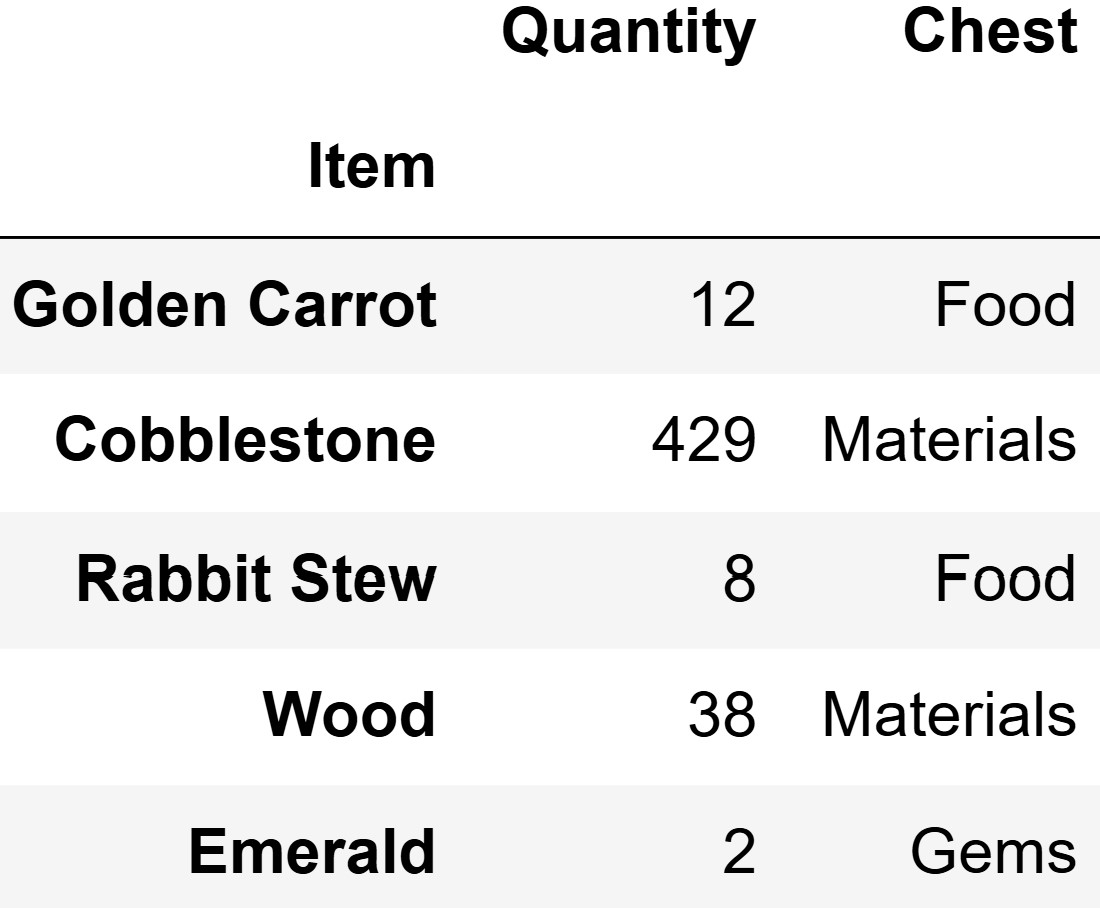
\includegraphics[width=1.8in]{quiz1df.jpg}
    \end{minipage}

\begin{probset}

\begin{prob}

Fill in the blanks so the expression below evaluates to the name of the chest that contains the most \textbf{distinct} items.

\begin{verbatim}
(items.groupby(___(a)___).___(b)___
      .sort_values(by="Quantity", ascending=___(c)___).___(d)___)
\end{verbatim}

\texttt{(a)}: \inlineresponsebox[2.6in]{\texttt{"Chest"}}{} \texttt{(b)}: \inlineresponsebox[2.6in]{\texttt{count()}}{}\\ \texttt{(c)}: \inlineresponsebox[2.6in]{\texttt{False}}{} \texttt{(d)}: \inlineresponsebox[2.6in]{\texttt{index[0]}}{}

\end{prob}

\bigskip


\begin{prob}

Steve wants to build a village where each house is built using a \textbf{different} \texttt{"Item"} from the \texttt{"Materials"} chest (e.g., a cobblestone house, a wood house, a brick house, etc). Assuming that each house requires at least 416 blocks of a single material, fill in the blanks so that the expression below evaluates to the \textbf{number of houses} that Steve's village will have.

\begin{verbatim}
items[(___(a)___) & (___(b)___)].___(c)___
\end{verbatim}

\vspace{1em}

\texttt{(a)}: \inlineresponsebox[6.5in]{\texttt{items.get("Chest") == "Materials"}}{}

\texttt{(b)}: \inlineresponsebox[6.5in]{\texttt{items.get("Quantity") >= 416}}{}

\texttt{(c)}: \inlineresponsebox[6.5in]{\texttt{shape[0]}}{} 

\end{prob}

\newpage

\begin{prob}
    Which of the following expressions evaluates to the number of \texttt{"Emerald"}s in Steve's chests? Select all that apply. 

    \smallskip

    \correctsquarebubble{\texttt{items.get("Quantity").loc["Emerald"]}}

    \smallskip
    
    \squarebubble{\texttt{(items[items.get("Item") == "Emerald"]}\\
    \hspace*{50pt}\texttt{.sort\_values(by="Quantity").loc["Emerald"])}}

    \smallskip
    \squarebubble{\texttt{items.sort\_values(by="Quantity").get("Quantity").iloc[0]}}

    \smallskip

    \correctsquarebubble{\texttt{items[items.index == "Emerald"].get("Quantity").iloc[0]}}

    \smallskip

    \squarebubble{None of the above.}

\end{prob}

\bigskip

\begin{prob}
    In early versions of Minecraft, players reported sighting a hazy figure with glowing eyes, who they nicknamed Herobrine. Examine the mysterious code that Herobrine left behind and determine the output. Write your answer \textbf{exactly} how the output would appear in Python. Do it wrong and your diamonds will disappear. 

    \noindent
\begin{minipage}{.5\textwidth}
\noindent 
    \begin{verbatim}
curse = 3 + 4 * 2 ** 2 - 6/3
curse
    \end{verbatim}
    \end{minipage}%
    \begin{minipage}{0.45\textwidth}
        \centering
        \inlineresponsebox[2in]{\texttt{17.0}}
    \end{minipage}
    
\end{prob}

\bigskip

\begin{prob}
    Below is the opening line from the legendary Minecraft parody song \emph{Revenge}:
    \begin{verbatim}
line = "Creeper aww man"
    \end{verbatim}  
    You want to create an echo effect to produce the following string:
    \begin{verbatim}
"Creeper Creeper Creeper aww man"
    \end{verbatim}  
Which of the following code snippets produces this output? Select all that apply.
    
    \smallskip
    
    \correctsquarebubble{ \texttt{words = line.split(" ")\\  
    \hspace*{20pt}(words[0] + " ") * 3 + words[1] + " " + words[2]}}
    
    \smallskip
    
    \squarebubble{ \texttt{line * 3}}
    
    \smallskip

    \correctsquarebubble{ \texttt{line.replace("Creeper", "Creeper Creeper Creeper")}}
    
    \smallskip
    
    \squarebubble{ \texttt{words = line.split(" ")\\  
    \hspace*{20pt}" ".join(words[0] * 3 + words[1])}}
    
    \smallskip

    \squarebubble{None of the above.}
\end{prob}


\end{probset}


\newpage

\begin{center}
\textbf{Reminders:}
\begin{itemize}
    \item \textbf{Write your PID} on the front page and on the top right corner of page 3.
    \item If your answer is a string, make sure to put it in \textbf{quotes}.
    \item If your answer is a float, make sure to include a \textbf{decimal point}.
    \item Stay in your seat until the quiz is over. No leaving early.
\end{itemize}
\end{center}

\end{document}
